\documentclass[usenames, dvipsnames, t]{beamer}

%\usepackage{geometry}
%\geometry{legalpaper, textwidth=426pt}
%\usepackage[T1]{fontenc}
%\usepackage{fourier}
\usepackage{graphicx}
%\graphicspath{{Figures/}}
%
\usepackage[english]{babel}															% English language/hyphenation
%\usepackage[protrusion=true,expansion=true]{microtype}
\usepackage{amsmath,amsfonts,amsthm} % Math packages
\usefonttheme[onlymath]{serif}
\usepackage{graphicx, adjustbox}
\graphicspath{{figures/}}

%\usepackage{url}
\newcommand{\red}[1]{\textcolor{red}{#1}}
\newcommand{\blue}[1]{\textcolor{blue}{#1}}
%
%% Self included packages
%%\usepackage[labelfont=sf,			hypcap=false,			format=hang,			width=\columnwidth]{caption}
%\usepackage{amsmath}
%\usepackage{wrapfig}
\usepackage[ruled, vlined]{algorithm2e}
\usepackage{pgfplots}
%\pgfplotsset{soldot/.style={color=blue,only marks,mark=*}} \pgfplotsset{holdot/.style={color=blue,fill=white,only marks,mark=*}}
\pgfplotsset{compat=1.12}
% \usepackage{subcaption}
\usepackage{xcolor}
\usepackage{tikz}
\usetikzlibrary{graphs, calc, graphs.standard, shapes.misc, positioning, fit, shadows, calc, snakes, shapes, patterns, arrows.meta, matrix, shapes.geometric}
% \usepackage[noend]{algpseudocode}
% \usetikzlibrary{external}
% \tikzexternalize[prefix=figures/tikz_externalize/]
\usepackage{hyperref}
\hypersetup{
    colorlinks,
    citecolor=black,
    filecolor=black,
    linkcolor=black,
    urlcolor=black
}
%\usepackage{ifthen}
\usepackage{bm}
%\usepackage{enumerate}
%%%%%%%%%%%%%%%%%%%%%%%%%%%%%%%%%%%%%%%%%%%%%%%%%%%%%%%%%%%%%%%%%%%%%%%%%%%
\usetheme{CambridgeUS}
\usecolortheme{beaver}
\usepackage[english]{babel}

\setbeamertemplate{section in toc}{\inserttocsection}
\setbeamertemplate{subsection in toc}{\hspace{1.2em}~\inserttocsubsection\par}

\setbeamerfont{section in toc}{size=\small}
\setbeamerfont{subsection in toc}{size=\footnotesize}

\setbeamertemplate{itemize item}{\color{red}$\circ$}
\setbeamertemplate{itemize subitem}{\color{red}$\circ$}

\setbeamertemplate{enumerate item}[default]
\setbeamercolor*{enumerate item}{fg=red}
\setbeamercolor*{enumerate subitem}{fg=red}
\setbeamercolor*{enumerate subsubitem}{fg=red}

\setbeamertemplate{footline}
{
  \leavevmode%
  \hbox{%
  \begin{beamercolorbox}[wd=.2\paperwidth,ht=2.25ex,dp=1ex,center]{author in head/foot}%
  	\usebeamerfont{author in head/foot}\insertshortauthor
  \end{beamercolorbox}%

  \begin{beamercolorbox}[wd=.5\paperwidth,ht=2.25ex,dp=1ex,center]{title in head/foot}%
    	\usebeamerfont{title in head/foot}\insertshorttitle\hspace*{3em}
  \end{beamercolorbox}%

  \begin{beamercolorbox}[wd=.3\paperwidth,ht=2.25ex,dp=1ex,right]{date in head/foot}%
    	\usebeamerfont{date in head/foot}\insertshortdate{}\hspace*{2em}
	\insertframenumber{} / \inserttotalframenumber\hspace*{2ex}
  \end{beamercolorbox}}%
  \vskip0pt%
}

\title[Interpolation of MD with Bi-Directional NN]{Interpolation of Molecular Dynamics Trajectories \\ with Bi-Directional Neural Networks}
\subtitle{}
\author[Winkler \& Sauceda]{Ludwig Winkler \& Huziel Sauceda}
\date{\today}


%%%%%%%%%%%%%%%%%%%%%%%%%%%%%%%%%%%%%%%%%%%%%%%%%%%%%%%%%%%%%%%%%%%%%%%%%%%%
\begin{document}

\def\mathn#1{\mathnormal{#1}}
\def\thet{\bm{\theta}}
\def\V{\mathn{V}}
\def\Q{\mathn{Q}}
\def\R{\mathn{R}}
\def\r{\mathn{r}}
\def\G{\mathn{G}}
\def\n{\mathn{n}}
\def\A{\mathn{A}}
\def\T{\mathn{T}}
\def\W{\mathn{W}}
% \def\E{\mathbb{E}}

\def\w{\mathn{w}}
\def\p{\mathn{p}}
\def\q{\mathn{q}}
\def\a{\mathn{a}}
\def\r{\mathn{r}}
\def\s{\mathn{s}}
\def\t{\mathn{t}}
\def\dist{1}

\newcommand{\E}{\mathbb{E}}

\tikzset{ shorten <>/.style={ shorten >=#1, shorten <=#1 } }


\begin{frame}
	\titlepage
\end{frame}

% \begin{frame}
% \frametitle{Outline}
% \tableofcontents
% \end{frame}

\begin{frame}
	\frametitle{Molecular Dynamics (MD)}
	\begin{itemize}
		\item<+-> "Classical" dynamics of molecules are governed by Newton's equations of motion 
		\item<+-> Position $r(t)$ and momentum $p(t)$ describe the system completely
		\item<+-> Dynamics $f$ given by differential equation
		\begin{align*}
			\dot{x}(t) =
			\begin{bmatrix}
				\dot{r}(t) \\ 
				\dot{p}(t)
			\end{bmatrix}
			= f \left(
			\begin{bmatrix}
				r(t) \\ 
				p(t)
			\end{bmatrix}
			,t
			\right)
		\end{align*}
		\onslide<+->
		\item Solution is a trajectory in phase space
		\begin{align*}
			x(t) = 
			\begin{bmatrix}
				r(t) \\ 
				p(t)
			\end{bmatrix}
			= 
			\int_{t_0}^t f \left( \begin{bmatrix} r(t) \\ p(t) \end{bmatrix} ,t \right) dt
		\end{align*}
	\end{itemize}
\end{frame}

\begin{frame}
	\frametitle{Molecular Dynamics (MD)}
	\begin{itemize}
		% \item<+-> Large N-body problems are expensive to solve
		\item<+-> High accuracy description of high dimensional N-bodies are expensive to compute
		\item<+-> MD requirements for a statistical meaningful result
		\begin{itemize}
			\item $\Delta t = 0.2 \ fs$ time step size for accurate integration of the equations of motion
			\item $T \sim 1 \ ns$: $10^6 - 10^7$ integration steps for expressive properties
		\end{itemize}
		\item<+-> Dynamics $f$ are expensive to solve for long simulations
		\item<+-> Single Thread DFT: $ 10 s $ integration step requires 110 days
		\item[] 
		\item<+-> Yet, essentially we are dealing with a time series prediction problem ...
		\item[] 
	\end{itemize}
	\onslide<+->
		\begin{center}
		\textbf{Can we learn the phase space dynamics with a ML algorithm?}
		\end{center}
\end{frame}

\begin{frame}
	\frametitle{Learning Dynamical Systems}
	\begin{itemize}
		\item<+-> Learn dynamics $f_\theta$ with NN from true dynamics $f$
		\item<+-> Integrate dynamics \red{$ \widehat{\dot{x}}(t) = f_\theta$} to obtain learned solution \red{$\hat{x}(t)$}
		\item<+-> Optimize $f_\theta$ to predict the true solutions $x(t)$
	\end{itemize}
	\onslide<+->
	% \begin{figure}[!htbp]
	% 	\begin{adjustbox}{max width = 0.3\textwidth, height = 0.6\textheight}
	% 		\begin{tikzpicture}
	% 			\tikzset{arrow/.style={-latex, shorten >= 5pt, shorten <= 5pt}}
	% 			\tikzset{diff/.style={-latex, shorten >= 5pt, shorten <= 5pt}}
	% 			\tikzset{node/.style={draw, circle, fill, scale=0.25}}
				
	% 			% \clip (-0.5,3) rectangle (10,-3);

	% 			\node (z0) [node]  at (0,-0.5) {}; 
	% 			\node (zT) [node, label={[above]{\scriptsize $x(t_0)$}}] at (5, 0.5) {};
		
	% 			\draw[arrow, black] (z0.north) .. controls +(45:5cm) and +(225:5cm) .. (zT);
	% 			\draw [decorate,decoration={brace,amplitude=10pt, mirror}, xshift=-4pt, yshift=0pt] (0,-1) -- (4.9,-1) node [black,midway,yshift=-0.6cm] {\large $x(t)$};

	% 			\onslide<5->{
	% 				\node[red, node, opacity=0] (t1) at (8, 0.8){};
	% 				\draw[red, dotted, arrow] (zT) to node[below, red] {\scriptsize $\widehat{\dot{x}}(t_0)$} (t1);
	% 			}
	% 			\onslide<6->{
	% 				\node[red, node, label={[above, red]{\scriptsize $x(t_1)$}}] (t1) at (8, 0.8){};
	% 			}
	% 			\onslide<7->{
	% 				\node[red, node, opacity=0] (t2) at (10, -0.5){};
	% 				\draw[red, dotted, arrow] (t1) to node[below left, red] {\scriptsize $\widehat{\dot{x}}(t_1)$} (t2);
	% 			}
	% 			\onslide<8->{
	% 				\node[red, node, label={[above right, red]{\scriptsize $x(t_2)$}}] (t2) at (10, -0.5){};
	% 			}
				
	% 			\onslide<9->{
	% 				\node[red, node, opacity=0] (t3) at (12, -0.4){};
	% 				\draw[red, dotted, arrow] (t2) to node[below, red] {\scriptsize $\widehat{\dot{x}}(t_2)$} (t3);
	% 			}
	% 			\onslide<10->{
	% 				\node[red, node, label={[above, red]{\scriptsize $x(t_3)$}}] (t2) at (12, -0.4){};
	% 			}

	% 			\onslide<11->{
				
	% 			\node[red, node] (t2) at (10, -0.5){};
	% 			\node[red, node] (t3) at (12, -0.4){};
				
	% 			\draw[red, dotted, arrow] (zT) to node[below, red] {} (t1);
	% 			% \draw[red, dotted, arrow] (t1) to node[above right, red] {$\widehat{\dot{x}}(t)$}  (t2);
	% 			\draw[red, dotted, arrow] (t2) to (t3);
		
	% 			\draw [red, decorate,decoration={brace,amplitude=10pt, mirror}, xshift=-4pt, yshift=0pt] (5.1,-1) -- (12.5,-1) node [red,midway,yshift=-0.6cm] {\large $\hat{x}(t)$};
	% 			}
	% 		\end{tikzpicture}
	% 	\end{adjustbox}
	% 	\end{figure}

	
	\begin{figure}[!htbp]
		\begin{adjustbox}{max width = 0.3\textwidth, height = 0.6\textheight}
			\begin{tikzpicture}[scale=2, line width = 0.05cm]

				\tikzset{simpoint/.style={circle, minimum width=7, inner sep=0, black, fill}}
				
				\draw [-latex, black] (0,-0.1) -- (0,2) node[at end, left] {};
				\draw [-latex, black] (-0.1,0) -- node[at end, below=0.5cm] {\large Time} (6.5,0);
			

				\onslide<4->{
				\node[simpoint] (t0) at (0.1,0.1){};
				\node[simpoint] (t1) at (1.5,1.5){};
				\node[simpoint] (t2) at (3.,0.25){};
				\node[simpoint] (t3) at (4.5,1.1){};
				\node[simpoint] (t4) at (6.,1.5){};
			
				% \draw[black] (t0) to (t1) to (t2) to (t3) to (t4);
				\draw[black, dashed] (t0) -- (t0 |- 0,0);
				\draw[black, dashed] (t1) -- (t1 |- 0,0);
				\draw[black, dashed] (t2) -- (t2 |- 0,0);
				\draw[black, dashed] (t3) -- (t3 |- 0,0);
				\draw[black, dashed] (t4) -- (t4 |- 0,0);

				\draw[{Bar[]}-{Bar[]}, ultra thick] (1.5, -0.25) -- node [below]{\large $\Delta t$} (3, -0.25);
				\node[above= 0.5cm of t2] () {\huge $x(t)$};
				}
				

				\onslide<5->{
				\draw [red] (0.1, 0.1)   to [out=60, in=180] (1.5,1.5)
				to [out=0, in=180] (3,0.25)
				to [out=0, in=135] (6,1.5)
				to [out=315, in=135] ++(315:0.5cm);

				\node[red, right= 0.75cm of t1] () {\huge $\hat{x}(t)$};
				\node[simpoint] (t0) at (0.1,0.1){};
				\node[simpoint] (t1) at (1.5,1.5){};
				\node[simpoint] (t2) at (3.,0.25){};
				\node[simpoint] (t3) at (4.5,1.1){};
				\node[simpoint] (t4) at (6.,1.5){};
				}

				\onslide<6->{
				\draw (4.25,0.9) rectangle ++(2,1);
				% \node[anchor=south west] (box) at (4.25,0.9) [draw,thick,minimum width=2pt,minimum height=1pt] {};
			
				\node[above= 4cm of t2] (zoom) {% <- this 'right of' is inherited; how to avoid?
				\begin{tikzpicture}[scale=3, line width = 0.05cm]
					\clip (4.25,0.9) rectangle ++(2,1.5);
					\draw[line width = 0.1cm] (4.25,0.9) rectangle ++(2,1.5);
					\draw [red] (0.1, 0.1)   to [out=0, in=180] (3,0.25)
													to [out=0, in=135] (6,1.5)
													to [out=315, in=135] ++(315:0.5cm);
			
					\node[simpoint] (t3) at (4.5,1.03){};
					\node[simpoint] (t4) at (6.,1.44){};
					\draw[black] (t3) to (t4);
			
					\draw[black] (4.5, 2.) to (6, 2.);
					\foreach \x in {4.5,5.,5.5,6.}
						\draw[black] (\x,1.9) -- (\x,2.1);
			
					\draw[red] (5, 2.) to (5.5, 2.);
					\foreach \x in {5.,5.5,}
						\draw[red] (\x,1.9) -- (\x,2.1);
					
					\node[red] at (5.25, 2.1) {$\Delta \tau$};
					\draw[black, dashed] (4.5, 2.0) |- (t3);
					\draw[black, dashed] (6, 2.0) |- (t4);
			
				\end{tikzpicture}
				};

				\draw ($(4.24, 0.9)+(0,1)$) -- ($(zoom.south west)+(0.1, 0.09)$);
				\draw ($(4.24, 0.9)+(2.01,1)$) -- ($(zoom.north east)+(-0.1, -0.08)$);
				}
			
			\end{tikzpicture}
		\end{adjustbox}
		\end{figure}
\end{frame}

\begin{frame}
	\frametitle{Learning Dynamical Systems}
	\framesubtitle{Model Architectures}
	\begin{itemize}	
		\item<+-> ODENetwork
		\begin{align*}
			\dot{x}(t) =
			\begin{bmatrix}
				\dot{r}(t) \\ 
				\dot{p}(t)
			\end{bmatrix}
			= f \left(
			\begin{bmatrix}
				r(t) \\ 
				p(t)
			\end{bmatrix}
			,t
			\right)
		\end{align*}
		\item<+-> HamiltonianNetwork
		\begin{align*}
			\dot{x}(t) = 
			\begin{bmatrix}
				\dot{r}(t) \\ \dot{p}(t)) 
			\end{bmatrix}
			= 
			\begin{bmatrix}
			\ \ \frac{\partial \mathcal{H}(r(t), p(t), t)}{\partial p(t)} \\ - \frac{\partial \mathcal{H}(r(t), p(t), t)}{\partial r(t)}
			\end{bmatrix}
		\end{align*}
		\item<+-> RNN and LSTM
		\begin{align*}
			\dot{x}(t) =
			\begin{bmatrix}
				\dot{r}(t) \\ 
				\dot{p}(t)
			\end{bmatrix}
			= f_\theta \left(
			\left[
			\begin{bmatrix}
				r(t_0) \\ 
				p(t_0)
			\end{bmatrix},
			\ldots, 
			\begin{bmatrix}
				r(t) \\ 
				p(t)
			\end{bmatrix}
			\right]
			,t
			\right)
		\end{align*}
	\end{itemize}
\end{frame}

\begin{frame}
	\frametitle{Learning Dynamical Systems with LSTM}
	\begin{itemize}
		\item<+-> Best performing due to fewest assumptions and flexible parameterization
		\item<+-> Memory cell $c(t)$ to selectively read and write information
		% \item<+-> Outputs $[ \dot{r}(t), \dot{p}(t)]^T$ are integrated to obtain solution $\hat{x}(t)$
	\end{itemize}
	\begin{figure}
		% \centering
		\begin{adjustbox}{max width = 1.\textwidth, height = 0.5\textheight}
			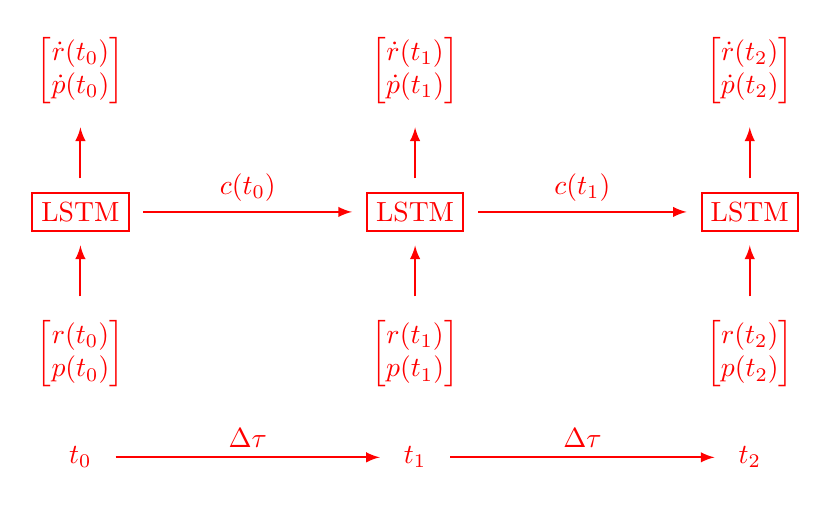
\begin{tikzpicture}[node distance=3cm, line width=0.025cm]
				\tikzset{arrow/.style={-latex, shorten >= 5pt, shorten <= 5pt}}
				% \tikzset{diff/.style={-latex, shorten >= 5pt, shorten <= 5pt}}
				% \tikzset{node/.style={draw, circle, fill, red, scale=0.25}}
				\tikzset{LSTMCell/.style={draw, rectangle, red, scale=1.}}
				% \tikzset{pics/little arrow/.style={code={
				% 		\draw[red,-latex] (0,0) arc[radius=0.4cm, start angle=90, end angle=360]
				% 		node[midway, red, fill=white,font=\scriptsize ]{#1};
				% 		}},
				% 		LSTMCell/.style={draw, rectangle, red, scale=1.,
				% 		append after command={([xshift=-0.0cm]\tikzlastnode.185)
				% 		pic{little arrow={#1}}
				% 		}}}

				% \clip (-3,-4) rectangle (10,3);
				
				% Step 0
				\onslide<4->{
				\node (lstm0) [LSTMCell] at (0,0) {LSTM}; 
				% \draw [-latex, red, draw] ([xshift=-0.0cm]lstm0.185) arc[radius=0.4cm, start angle=90, end angle=360] node[midway, red, fill=white](){\scriptsize $c(t)$};
				

				\node (input0) [red, below = 1cm of lstm0] {$\begin{bmatrix} r(t_0) \\ p(t_0) \end{bmatrix}$};
				\draw [arrow, red] (input0) -- (lstm0);
				\node (output0) [red, above = 1cm of lstm0] {$\begin{bmatrix} \dot{r}(t_0) \\ \dot{p}(t_0) \end{bmatrix}$};
				\draw [arrow, red] (lstm0) -- (output0);

				\node (t0)[red, below=0.5cm of input0]{$t_0$};
				}
				
				\onslide<5->{
					\node (lstm1) [opacity=0, right = of lstm0] {LSTM}; 
					\node (input1) [opacity=0, below = 1cm of lstm1] {$\begin{bmatrix} r(t_1) \\ p(t_1) \end{bmatrix}$};
					\node (t1)[red, below=0.5cm of input1]{$t_1$};
					\draw [arrow, red] (t0) -- node[above]{$\Delta \tau$} (t1);
				}

				\onslide<6->{
					\node (lstm1) [LSTMCell, right = of lstm0] {LSTM}; 
					\node (input1) [red, below = 1cm of lstm1] {$\begin{bmatrix} r(t_1) \\ p(t_1) \end{bmatrix}$};
					\draw [arrow, red] (input1) -- (lstm1);
					\node (output1) [red, above = 1cm of lstm1] {$\begin{bmatrix} \dot{r}(t_1) \\ \dot{p}(t_1) \end{bmatrix}$};
					\draw [arrow, red] (lstm1) -- (output1);
				}

				\onslide<7->{
					\draw [arrow, red] (lstm0) -- node[above]{$c(t_0)$} (lstm1);
				}

				\onslide<8->{
					\node (lstm2) [opacity=0, right = of lstm1] {LSTM}; 
					\node (input2) [opacity=0, below = 1cm of lstm2] {$\begin{bmatrix} r(t_1) \\ p(t_1) \end{bmatrix}$};
					\node (t2)[red, below=0.5cm of input2]{$t_2$};
					\draw [arrow, red] (t1) -- node[above]{$\Delta \tau$} (t2);
				}

				\onslide<9->{
					\node (lstm2) [LSTMCell, right = of lstm1] {LSTM}; 
					\node (input2) [red, below = 1cm of lstm2] {$\begin{bmatrix} r(t_2) \\ p(t_2) \end{bmatrix}$};
					\draw [arrow, red] (input2) -- (lstm2);
					\node (output2) [red, above = 1cm of lstm2] {$\begin{bmatrix} \dot{r}(t_2) \\ \dot{p}(t_2) \end{bmatrix}$};
					\draw [arrow, red] (lstm2) -- (output2);
				}

				\onslide<10->{
					\draw [arrow, red] (lstm1) -- node[above]{$c(t_1)$} (lstm2);
				}
				

				% \onslide<5->{
				% \node (lstm1) [LSTMCell, right = of lstm0] {LSTM}; 
				% % \draw [-latex, red, draw] ([xshift=-0.0cm]lstm1.185) arc[radius=0.4cm, start angle=90, end angle=360] node[midway, red, fill=white](){\scriptsize $c(t)$};
				% \draw [arrow, red] (t0) -- node[above]{$\Delta t$} (t1);
				% \node (t1)[red, below=0.5cm of input1]{$t_1$};
				% }

				% \node (input1) [red, below = 1cm of lstm1] {$\begin{bmatrix} r(t_1) \\ p(t_1) \end{bmatrix}$};
				
				% \node (output1) [red, above = 1cm of lstm1] {$\begin{bmatrix} \dot{r}(t_1) \\ \dot{p}(t_1) \end{bmatrix}$};
				% \draw [arrow, red] (lstm1) -- (output1);

				% \node (lstm2) [LSTMCell, right = of lstm1] {LSTM}; 
				% % \draw [-latex, red, draw] ([xshift=-0.0cm]lstm2.185) arc[radius=0.4cm, start angle=90, end angle=360] node[midway, red, fill=white](){\scriptsize $c(t)$};
			
				% \node (input2) [red, below = 1cm of lstm2] {$\begin{bmatrix} r(t_2) \\ p(t_2) \end{bmatrix}$};
				% \draw [arrow, red] (input2) -- (lstm2);
				% \node (output2) [red, above = 1cm of lstm2] {$\begin{bmatrix} \dot{r}(t_2) \\ \dot{p}(t_2) \end{bmatrix}$};
				% \draw [arrow, red] (lstm2) -- (output2);

				% % Recurrent connections
				% \draw [arrow, red] (lstm0) -- node[above]{$c(t)$} (lstm1);
				% \draw [arrow, red] (lstm1) -- node[above]{$c(t)$} (lstm2);
				
				% % Time Steps
				% \node (t1)[red, below=0.5cm of input1]{$t_1$};
				% \node (t2)[red, below=0.5cm of input2]{$t_2$};
				% \onslide<4->{\draw [arrow, red] (t0) -- node[above]{$\Delta t$} (t1);}
				% \onslide<5->{\draw [arrow, red] (t1) -- node[above]{$\Delta t$} (t2);}
			
			\end{tikzpicture}
		% }
		\end{adjustbox}
	\end{figure}
\end{frame}

\begin{frame}
	\frametitle{Bi-Directional Interpolation of Differential Equation}
	\begin{itemize}
		% \item<+-> Analytical simulation provides most accurate solution
		% \item<+-> Combine speed of ML-MD with accuracy of analytical MD
		\item<+-> Use coarse, analytical MD to provide initial and final conditions
		\item<4-> Integrate dynamics \red{forward} \onslide<5-> and \blue{backward} through time
	\end{itemize}
	\onslide<+->
	% \begin{figure}[!htbp]
	% 	\begin{adjustbox}{max width = 0.3\textwidth, height = 0.4\textheight}
	% 		\begin{tikzpicture}
	% 			\tikzset{arrow/.style={-latex, shorten >= 5pt, shorten <= 5pt}}
	% 			\tikzset{diff/.style={-latex, shorten >= 5pt, shorten <= 5pt}}
	% 			\tikzset{node/.style={draw, circle, fill, scale=0.25}}
				
	% 			% \node (z0) [node, label={[below, black]{$x(t)$}}] at (0,-0.5) {}; 
	% 			\node (z0) [node]  at (0,-0.5) {}; 
	% 			\node (zT) [node] at (5, 0.5) {};
		
	% 			\draw[arrow, black] (z0.north) .. controls +(45:5cm) and +(225:5cm) .. node[below left]{$x(t)$} (zT);
	% 			\draw [decorate,decoration={brace,amplitude=10pt, mirror}, xshift=-4pt, yshift=0pt] (0,-1) -- (4.9,-1) node [black,midway,yshift=-0.6cm] {$\text{Initial Condition} \rightarrow $};
				
	% 			\node (zT1) at (10, -0.5) {};
	% 			\draw[draw=none] (zT.north) .. controls +(50:3cm) and +(225:3cm) .. node[above right, red]{$\hat{x}(t)$} (zT1)
	% 			\foreach \t in {33,66,100}
	% 			{ node[red] (a\t) [pos=\t/100,node,draw=red] {} };
				
	% 			\draw[red, dotted, arrow] (zT) to node[below, red] {} (a33);
	% 			\draw[red, dotted, arrow] (a33) to node[below left, red] {} (a66);
	% 			\draw[red, dotted, arrow] (a66) to (a100);
		
	% 			% \node (reala100)[node] at ($(a100)+(0,1.0)$) {};
	% 			% \draw[black, dotted, arrow, shorten >= 2pt] (a66) to node[above, black] {\scriptsize $dx(t)$} (reala100);
	% 			% \draw[{Bar[]}-{Bar[]}, red, dashed, shorten >= 3pt, shorten <= 3pt] (a100) to node[right]{$\mathcal{L}$} (reala100);
	% 			\draw [red, decorate,decoration={brace,amplitude=10pt, mirror}, xshift=-4pt, yshift=0pt] (5.1,-1) -- (10,-1) node [red,midway,yshift=-0.6cm] {ML-MD Prediction};
		
	% 			\node (zT2)[node] at (14, 1) {};
	% 			\draw[arrow, black] (a100.east) .. controls +(20:2cm) and +(135:2cm) .. node[above left] {$x(t)$} (zT2);
	% 			\draw [decorate,decoration={brace,amplitude=10pt, mirror}, xshift=-4pt, yshift=0pt] (10.1,-1) -- (13.9,-1) node [black,midway,yshift=-0.6cm] {$\leftarrow \text{Final} \ \ | \ \text{Initial} \rightarrow$};
				
	% 			\node (zT3) [label={[above=0.1cm, red]{$x(t)$}}] at (18, 0.5) {};
	% 			\draw[draw=none] (zT2.north) .. controls +(300:3cm) and +(225:3cm) .. node[above right, red]{} (zT3)
	% 			\foreach \t in {33,66,100}
	% 			{ node[red] (b\t) [pos=\t/100,node,draw=red] {} };
				
	% 			% \draw[red, dotted, arrow] (zT2) to node[above right, red] {123} (b33);
	% 			\draw[red, dotted, arrow] (zT2) to (b33);
	% 			\draw[red, dotted, arrow] (b33) to (b66);
	% 			\draw[red, dotted, arrow] (b66) to (b100);
		
	% 			\draw [red, decorate,decoration={brace,amplitude=10pt, mirror}, xshift=-4pt, yshift=0pt] (14.1,-1) -- (18.1,-1) node [red,midway,yshift=-0.6cm] {ML-MD Prediction};
	% 		\end{tikzpicture}
	% 	\end{adjustbox}
	% 	\end{figure}	
	\begin{figure}[!htbp]
		\begin{adjustbox}{max width = 0.3\textwidth, height = 0.5\textheight}
			\begin{tikzpicture}[scale=2, line width = 0.05cm]
				\tikzset{simpoint/.style={circle, minimum width=7, inner sep=0, black, fill}}
				
				\draw [-latex, black] (0,-0.1) -- (0,2) node[at end, left] {};
				\draw [-latex, black] (-0.1,0) -- node[at end, below=0.5cm] {\large Time} (6.5,0);
			

				\onslide<2->{
					\node[simpoint] (t0) at (0.1,0.1){};
					\node[simpoint] (t1) at (1.5,1.5){};
					\node[simpoint] (t2) at (3.,0.25){};
					\node[simpoint] (t3) at (4.5,1.1){};
					\node[simpoint] (t4) at (6.,1.5){};
				
					% \draw[black, thick] (t0) to (t1) to (t2) to (t3) to (t4);
					\draw[black, dashed] (t0) -- (t0 |- 0,0);
					\draw[black, dashed] (t1) -- (t1 |- 0,0);
					\draw[black, dashed] (t2) -- (t2 |- 0,0);
					\draw[black, dashed] (t3) -- (t3 |- 0,0);
					\draw[black, dashed] (t4) -- (t4 |- 0,0);

					\draw[{Bar[]}-{Bar[]}, ultra thick] (1.5, -0.25) -- node [below]{\large $\Delta t$} (3, -0.25);
					\node[above= 0.5cm of t2] () {\huge $x(t)$};
				
					\draw [red] (0.1, 0.1)   to [out=60, in=180] (1.5,1.5)
					to [out=0, in=180] (3,0.25)
					to [out=0, in=135] (6,1.5)
					to [out=315, in=135] ++(315:0.5cm);

					\node[red, right= 0.75cm of t1] () {\huge $\hat{x}(t)$};
					% \draw[black] (t0) to (t1) to (t2) to (t3) to (t4);
					\node[simpoint] (t0) at (0.1,0.1){};
					\node[simpoint] (t1) at (1.5,1.5){};
					\node[simpoint] (t2) at (3.,0.25){};
					\node[simpoint] (t3) at (4.5,1.1){};
					\node[simpoint] (t4) at (6.,1.5){};
				}

				\onslide<3->{
					\draw (4.25,0.9) rectangle ++(2,1);
					% \node[anchor=south west] (box) at (4.25,0.9) [draw,thick,minimum width=2pt,minimum height=1pt] {};
				
					\node[above= 4cm of t2] (zoom) {% <- this 'right of' is inherited; how to avoid?
					\begin{tikzpicture}[scale=3, line width=0.05cm]
						
						\clip (4.25,0.9) rectangle ++(2,1.5);
						\draw[line width = 0.1cm] (4.25,0.9) rectangle ++(2,1.5);
						\draw [red] (0.1, 0.1)   to [out=0, in=180] (3,0.25)
														to [out=0, in=135] (6,1.5)
														to [out=315, in=135] ++(315:0.5cm);
				
						\node[simpoint] (t3) at (4.5,1.03){};
						\node[simpoint] (t4) at (6.,1.44){};
						\draw[black] (t3) to (t4);
						
						\onslide<4->{
							\draw [red, yshift=0.2cm, -latex] 
							(4.5,1.0) to [out=45, in=220] (5.,1.45);
						}
						\onslide<5->{
							\draw [blue, -latex] (6, 1.6) to [out=135, in=0] (5.5,1.8);
						}
				
						\draw[black] (4.5, 2.) to (6, 2.);
						\foreach \x in {4.5,5.,5.5,6.}
							\draw[black] (\x,1.9) -- (\x,2.1);
				
						\draw[red] (5, 2.) to (5.5, 2.);
						\foreach \x in {5.,5.5,}
							\draw[red] (\x,1.9) -- (\x,2.1);
						
						\node[red] at (5.25, 2.1) {$\Delta \tau$};
						\draw[black, dashed] (4.5, 2.0) |- (t3);
						\draw[black, dashed] (6, 2.0) |- ($(t4)+(0, -0.1)$);
				
					\end{tikzpicture}
				};
				
				\draw ($(4.24, 0.9)+(0,1)$) -- ($(zoom.south west)+(0.1, 0.09)$);
				\draw ($(4.24, 0.9)+(2.01,1)$) -- ($(zoom.north east)+(-0.1, -0.08)$);
				}
			
			\end{tikzpicture}
		\end{adjustbox}
		\end{figure}
\end{frame}

\begin{frame}
	\frametitle{Bi-Directional Interpolation of Differential Equation}
	\begin{itemize}
		\item<+-> Predict \red{forward solution $\overrightarrow{\hat{x}(t)}$} and \blue{backward solution $\overleftarrow{\hat{x}(t)}$} with the \textbf{same} dynamics $f_\theta$
		\item<+-> Use adiabatic connection to interpolate \red{$\overrightarrow{\hat{x}(t)}$} and \blue{$\overleftarrow{\hat{x}(t)}$} to $\hat{x}(t)$
		\onslide<+->
		\begin{align}
			\hat{x}(t) = (1-\lambda(t)) \ \red{\overrightarrow{\hat{x}(t)}} + \lambda(t) \ \blue{\overleftarrow{\hat{x}(t)}}
		\end{align}
	\end{itemize}
	% \resizebox*{0.5\textwidth}{1.2\textheight}{
	\begin{figure}
		% \centering
		\begin{adjustbox}{max width = 1.\textwidth, height = 0.5\textheight}
			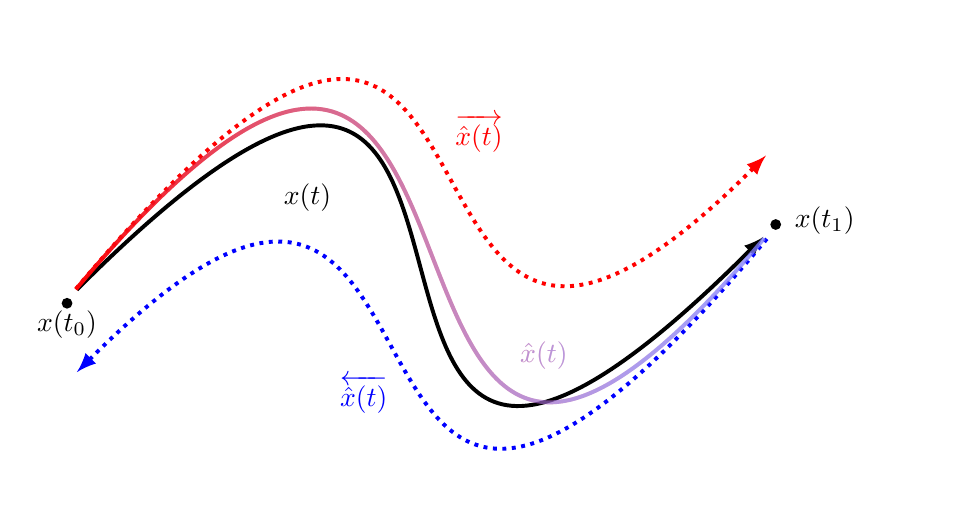
\begin{tikzpicture}[line width= 0.05cm]
			\tikzset{arrow/.style={-latex, shorten >= 5pt, shorten <= 5pt}}
			\tikzset{diff/.style={-latex, shorten >= 5pt, shorten <= 5pt}}
			\tikzset{node/.style={draw, circle, fill, scale=0.25}}

			\clip (-0.5,3) rectangle (11,-3);

			\onslide<4->{
			
			\node (z0) [node, label={[below]{$x(t_0)$}}] at (0,-0.5) {}; 
			\node (zT) [node, label={[right=0.1cm]{$x(t_1)$}}] at (9, 0.5) {};
			\draw[arrow, black] (z0.north) .. controls +(45:10cm) and +(225:10cm) .. node[above left = 0.5cm and ]{$x(t)$} (zT);
			}
			
			\onslide<5->{
			\draw[arrow, dotted, red] (z0.north) .. controls +(50:10cm) and +(225:8cm) .. node[above right]{$\overrightarrow{\hat{x}(t)}$} ($(zT)+(0cm,1cm)$);
			}
			\onslide<6->{
			\draw[arrow, dotted, blue] (zT.south) .. controls +(230:10cm) and +(45:8cm) .. node[below left]{$\overleftarrow{\hat{x}(t)}$}($(z0)+(0cm,-1cm)$);
			}

			\onslide<7->{
			\draw[shorten >= 5pt, shorten <= 5pt, red, path fading=east] (z0.north) .. controls +(50:10cm) and +(230:9.5cm) .. node[below right = 1cm and 1cm]{$\hat{x}(t)$} (zT);
			\draw[shorten >= 5pt, shorten <= 5pt, blue!50, path fading=west, opacity=0.8] (z0.north) .. controls +(50:10cm) and +(230:9.5cm) .. node[below right = 1cm and 1cm]{$\hat{x}(t)$} (zT);
			}

			\end{tikzpicture}
		% }
		\end{adjustbox}
	\end{figure}
\end{frame}

\begin{frame}
	\frametitle{Bi-Directional Interpolation of Differential Equation}
	\begin{itemize}
		\item For time-reversible solutions, we obtain
		\begin{align*}
			\hat{x}(t) &= (1-\lambda(t)) \ \overrightarrow{\hat{x}(t)} + \lambda(t) \ \overleftarrow{\hat{x}(t)} \\
			&= \underbrace{(1-\lambda(t)) x(t_0) + \lambda(t) x(t_1)}_{\text{low frequency components}} + \underbrace{\int_{t=t_0}^{t_1} f_\theta \left(x(t), t \right) dt }_{\text{high frequency components}}
		\end{align*}
		\item<+-> Adiabatic connection frees the ML model to model high frequency signals
	\end{itemize}
	\begin{figure}[!htbp]
		\begin{adjustbox}{max width = 0.3\textwidth, height = 0.3\textheight}
			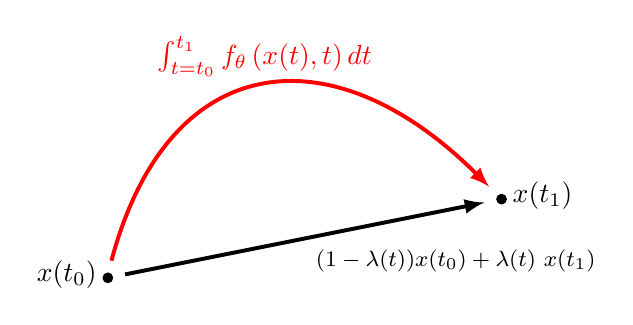
\begin{tikzpicture}[line width= 0.05cm]
				\tikzset{arrow/.style={-latex, shorten >= 5pt, shorten <= 5pt}}
				\tikzset{diff/.style={-latex, shorten >= 5pt, shorten <= 5pt}}
				\tikzset{node/.style={draw, circle, fill, scale=0.25}}
				
				% \node (z0) [node, label={[below, black]{$x(t)$}}] at (0,-0.5) {}; 
				\node (z0) [node, label={[left] {$x(t_0)$}}]  at (0,0) {}; 
				\node (zT) [node, label={[right] {$x(t_1)$}}] at (5, 1) {};
		
				\draw[arrow, red] (z0.north) .. controls +(75:3cm) and +(135:3cm) .. node[above, red]{$\int_{t=t_0}^{t_1} f_\theta \left(x(t), t \right) dt$} (zT);
				% \draw [decorate,decoration={brace,amplitude=10pt, mirror}, xshift=-4pt, yshift=0pt] (0,-1) -- (4.9,-1) node [black,midway,yshift=-0.6cm] {$\text{Initial Condition} \rightarrow $};
				\draw [arrow] (z0) -- node[below right]{\footnotesize $(1-\lambda(t)) x(t_0) + \lambda(t) \ x(t_1)$} (zT);
			\end{tikzpicture}
		\end{adjustbox}
		\end{figure}
\end{frame}

\begin{frame}
	\frametitle{Uni-Directional Interpolation of Differential Equation}
	\begin{itemize}
		 \item Unidirectional LSTM architecture for Benzene MD trajectory interpolating over 20 time steps
	\end{itemize}
	\begin{figure}
		 \centering
		 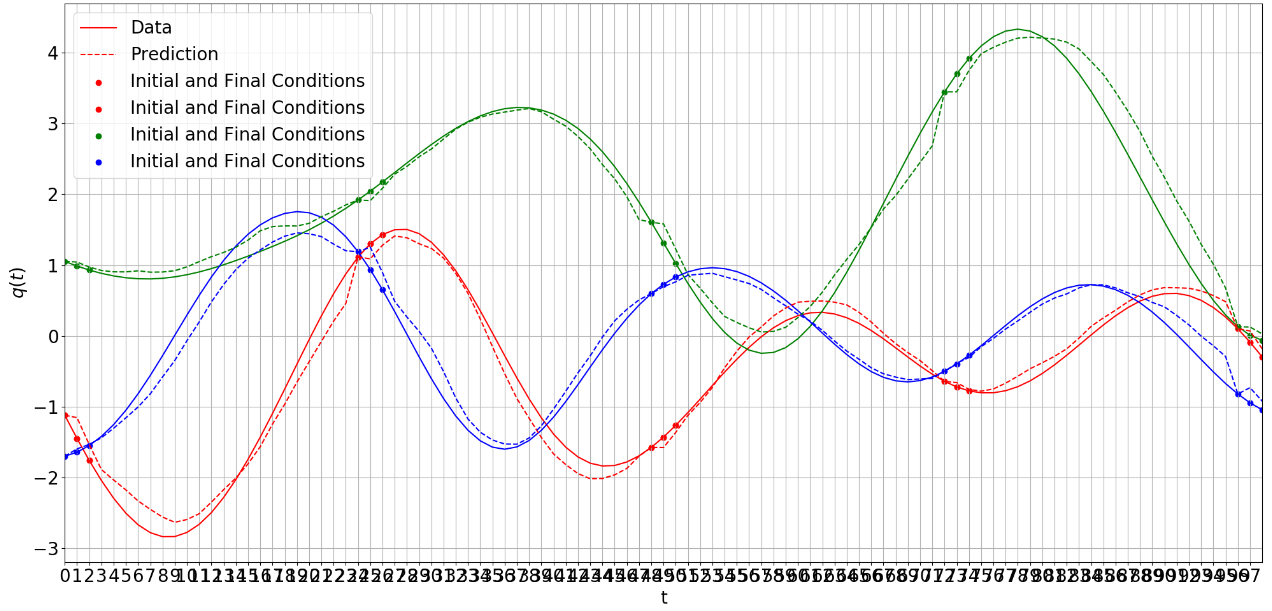
\includegraphics[width=0.8\textwidth]{ExampleTrajectory.png}
	\end{figure}
\end{frame}

\begin{frame}
	\frametitle{Bi-Directional Interpolation of Differential Equation}
	\begin{itemize}
		 \item Bidirectional LSTM architecture for Benzene MD trajectory interpolating over 20 time steps
		 \item Final condition and additional bidirectional training smooth trajectories significantely
	\end{itemize}
	\begin{figure}
		 \centering
		 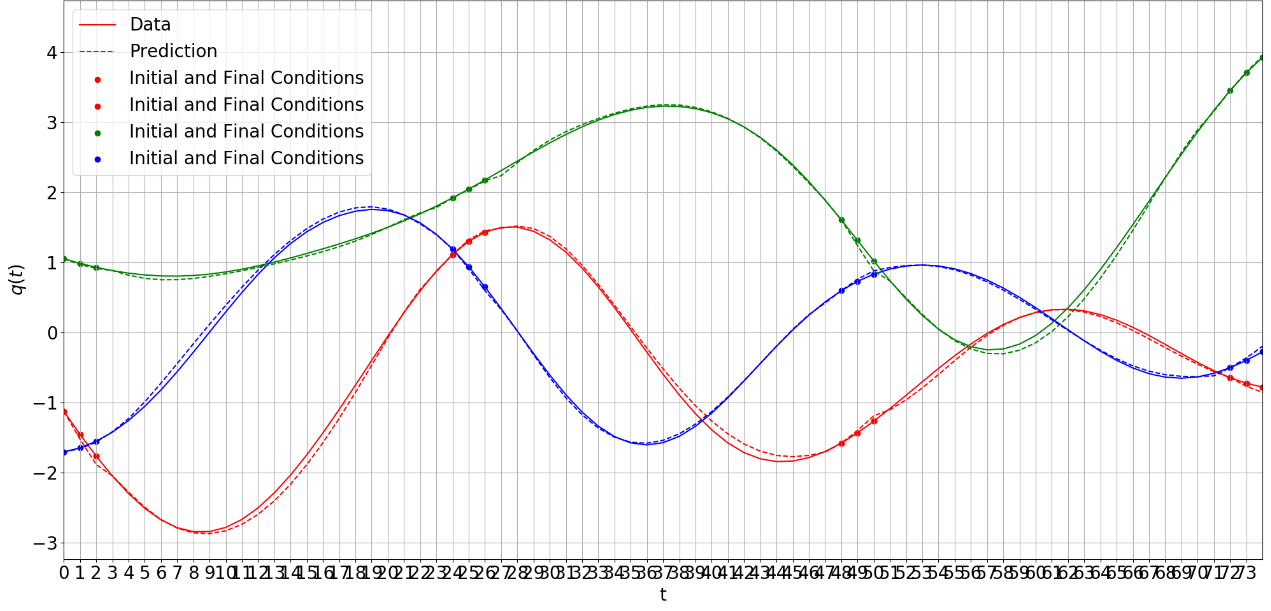
\includegraphics[width=0.8\textwidth]{ExampleTrajectoryBi.png}
	\end{figure}
\end{frame}

\begin{frame}
	\frametitle{Bi-Directional Interpolation of Differential Equation}
	\begin{itemize}
		 \item Single initial and final condition already good for sufficient performance by bidirectional LSTM
	\end{itemize}
	\begin{figure}
		 \centering
		 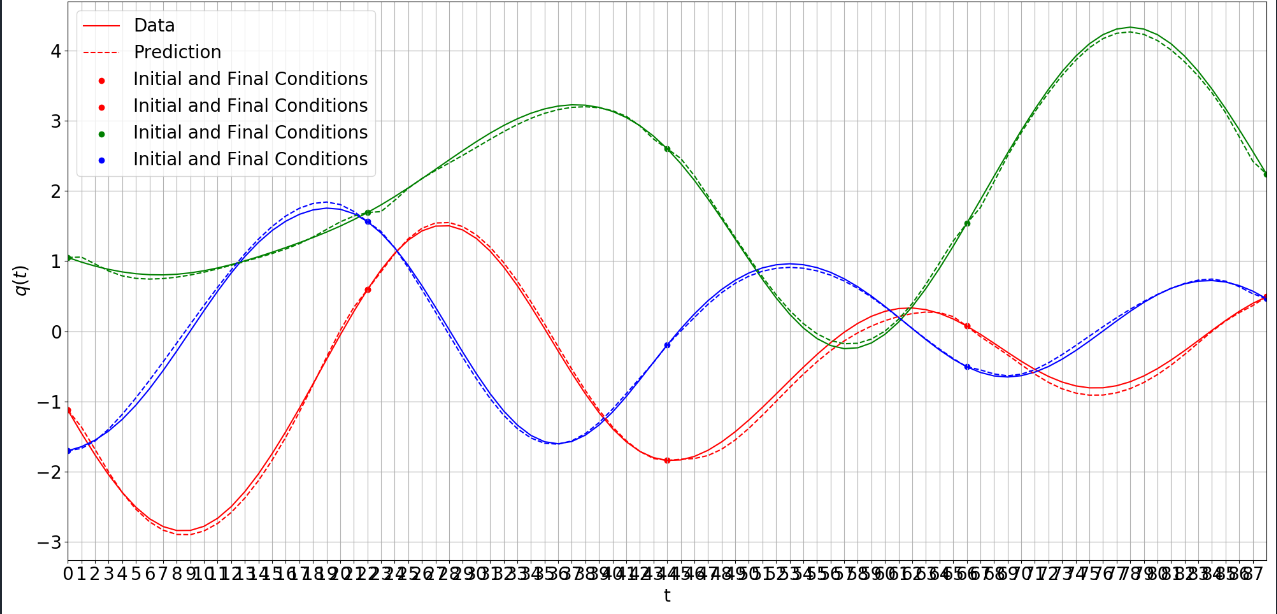
\includegraphics[width=0.8\textwidth]{ExampleTrajectoryBiIn1.png}
	\end{figure}
\end{frame}

\begin{frame}
	\frametitle{Analysis of Interpolations}
	\begin{figure}[htb]
		\begin{minipage}{0.3\textwidth}
			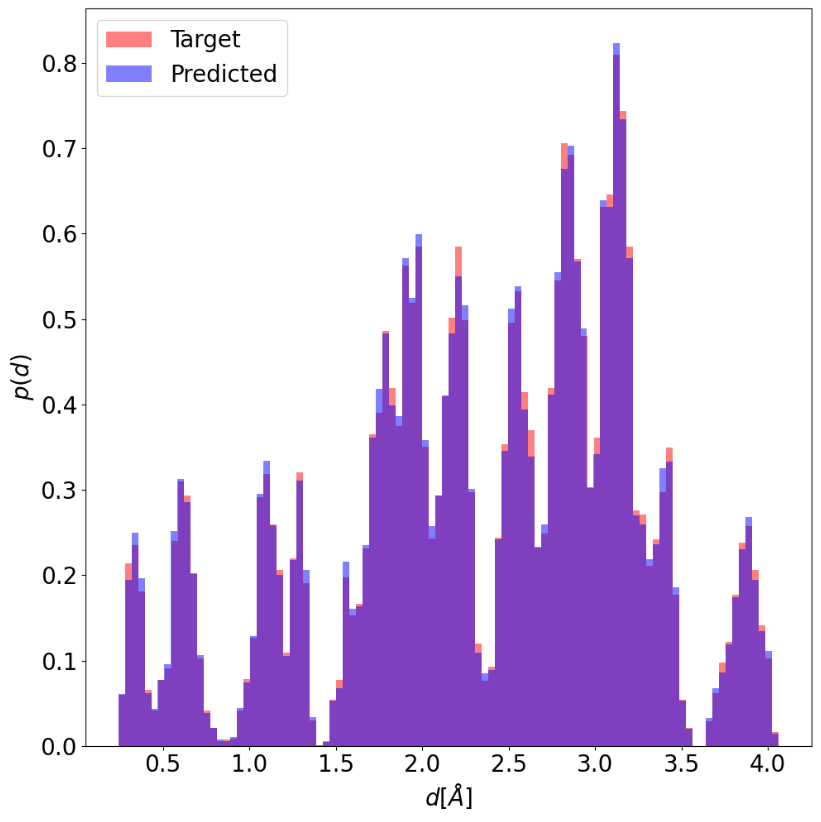
\includegraphics[width=0.9\linewidth, height=5cm]{KetoMalonaldehyde100K_BiLSTM.png} 
			\caption{Keto-Malondialdehyde ($100K$)}
		\end{minipage}
		\begin{minipage}{0.3\textwidth}
			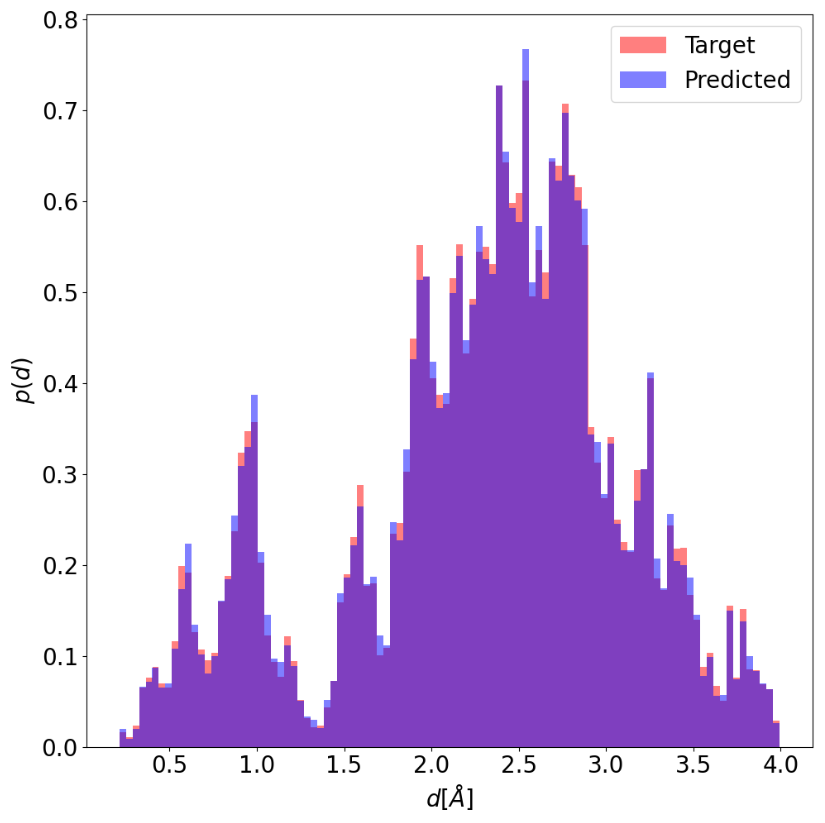
\includegraphics[width=0.9\linewidth, height=5cm]{KetoMalonaldehyde300K_BiLSTM.png}
			\caption{Keto-Malondialdehyde ($300K$)}
		\end{minipage}
		\begin{minipage}{0.3\textwidth}
			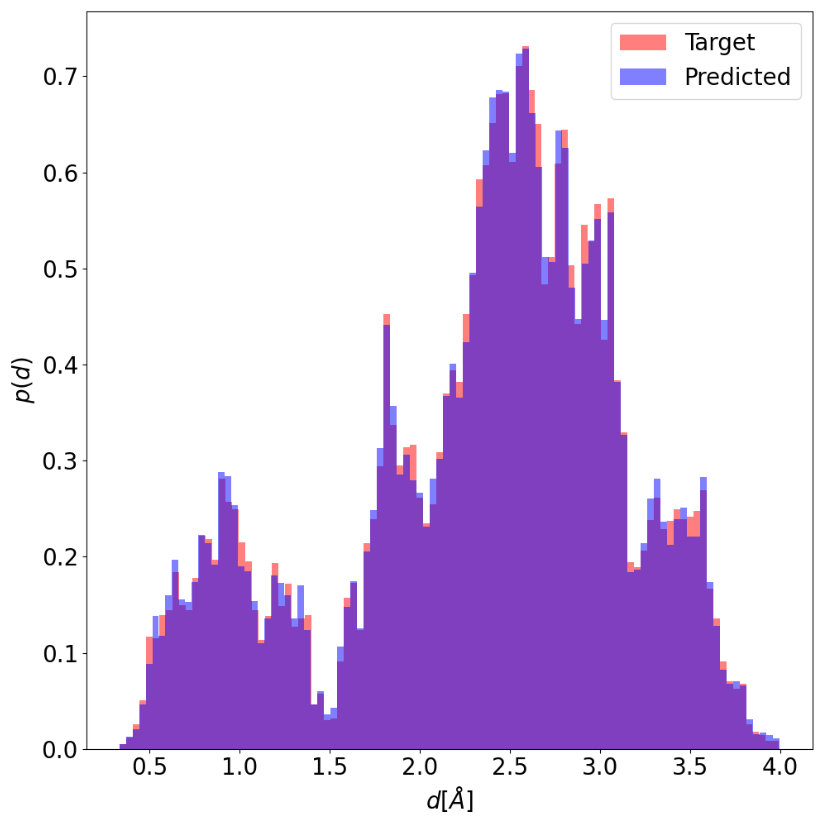
\includegraphics[width=0.9\linewidth, height=5cm]{KetoMalonaldehyde500K_BiLSTM.png}
			\caption{Keto-Malondialdehyde ($500K$)}
		\end{minipage}
		% \caption{The distribution of interatomic distances $d$[ \AA ] of Keto-Malonaldehyde at 100 Kelvin (K), 300 Kelvin and 500 Kelvin. The predicted distribution of interatomistic distances is shown in red and the target distribution is shown in blue. The distributions becomes less multi-modal as the temperature increases.}
		% \label{fig:interatomisticdistances}
	\end{figure}
\end{frame}

\begin{frame}
	\frametitle{Analysis of Interpolations}
	\begin{figure}[htb]
		\begin{minipage}{0.49\textwidth}
			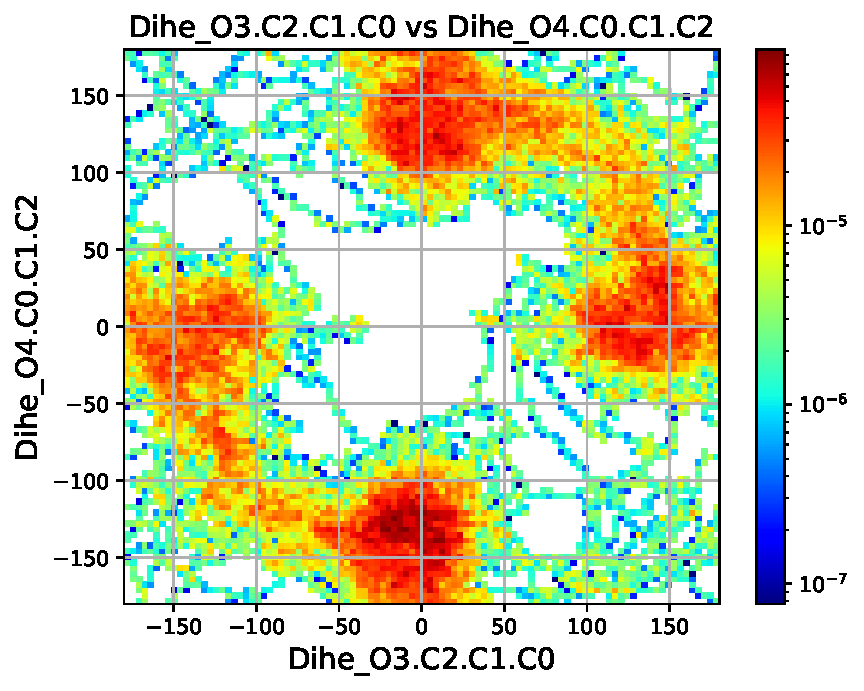
\includegraphics[width=0.9\linewidth, height=5cm]{KETO-MDA_300K_GroundTruth.pdf} 
			\caption{Ground Truth Free Energy Keto-Malondialdehyde ($300K$)}
		\end{minipage}
		\begin{minipage}{0.49\textwidth}
			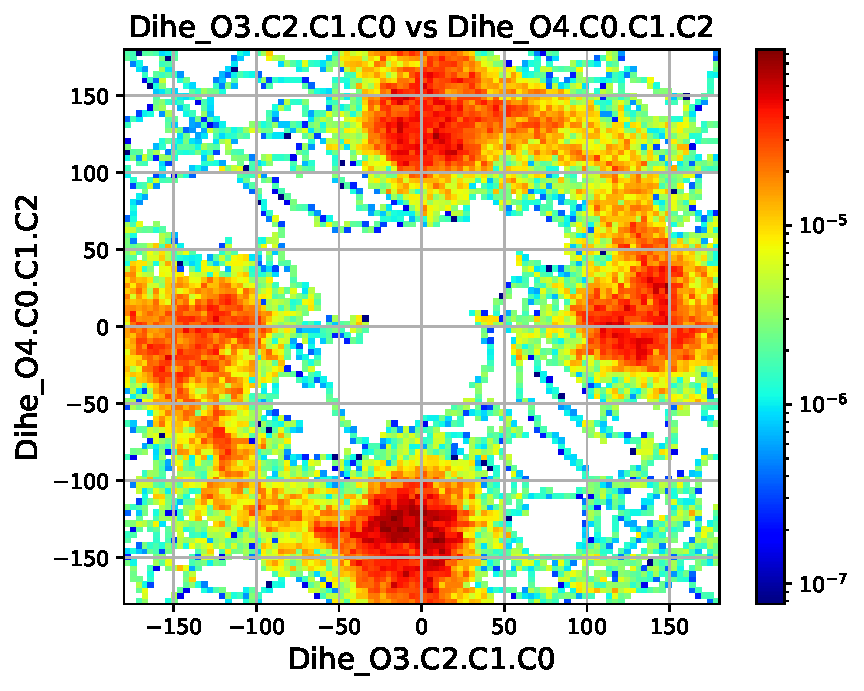
\includegraphics[width=0.9\linewidth, height=5cm]{KETO-MDA_300K_ML.pdf}
			\caption{Predicted Free Energy Keto-Malondialdehyde ($300K$)}
		\end{minipage}
		% \caption{I don't know how to interpret these plots ...}
		% \label{fig:interatomisticdistances}
	\end{figure}
\end{frame}

\begin{frame}
	\frametitle{Future Work}
	\begin{itemize}
		\item<+-> Adaptively switch between simulation and ML prediction
		\item<+-> Leverage speed of ML prediction for smooth sub-trajectories
		\item<+-> Regularly monitor ML prediction performance with parallel simulation 
	\end{itemize}
	\begin{figure}[!htbp]
		\begin{adjustbox}{max width = 0.3\textwidth, height = 0.4\textheight}
			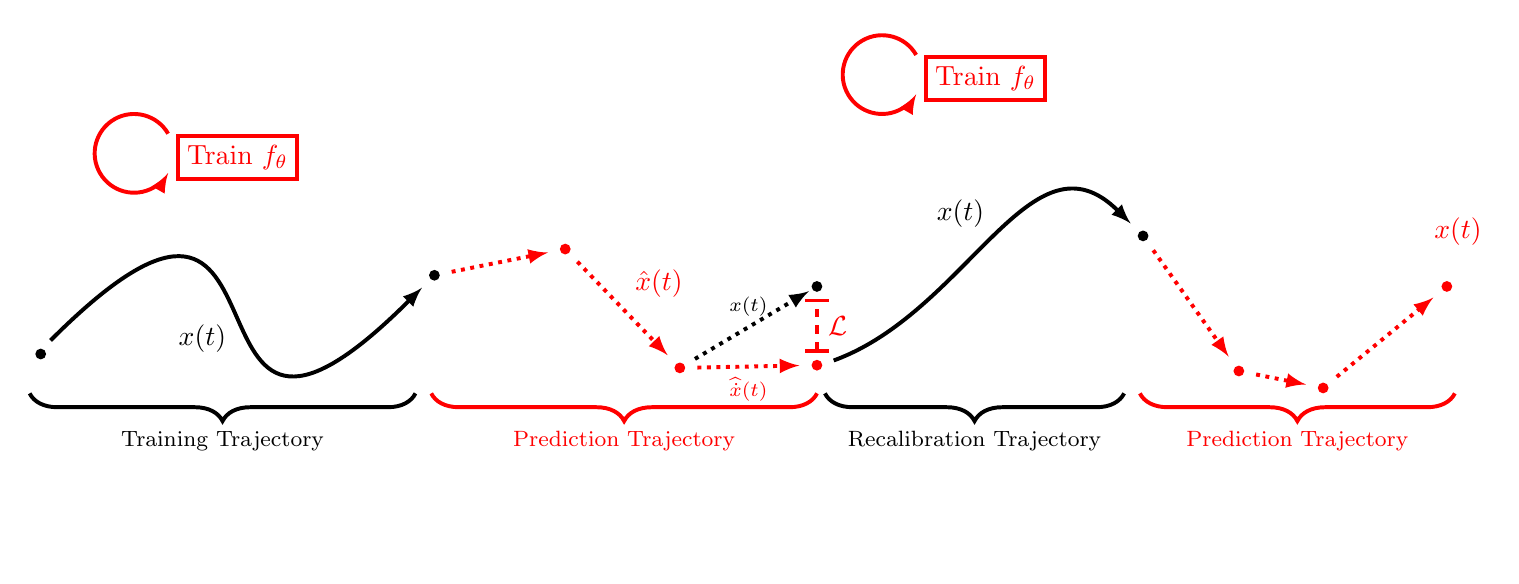
\begin{tikzpicture}[line width= 0.05cm]
				\tikzset{arrow/.style={-latex, shorten >= 5pt, shorten <= 5pt}}
				\tikzset{diff/.style={-latex, shorten >= 5pt, shorten <= 5pt}}
				\tikzset{node/.style={draw, circle, fill, scale=0.25}}
				
				\onslide<4->{
				\node (z0) [node]  at (0,-0.5) {}; 
				\node (zT) [node] at (5, 0.5) {};
		
				\draw[arrow, black] (z0.north) .. controls +(45:5cm) and +(225:5cm) .. node[below left]{$x(t)$} (zT);
				\draw [decorate,decoration={brace,amplitude=10pt, mirror}, xshift=-4pt, yshift=0pt] (0,-1) -- (4.9,-1) node [black,midway,yshift=-0.6cm] {\footnotesize Training Trajectory};
				}

				\onslide<5->{
					\node[red, rectangle, draw] at (2.5, 2) (train1) {Train $f_\theta$};
					\draw [-latex, red] ([xshift=-0.1cm]train1.north west) arc[radius=0.5cm, start angle=30, end angle=330];
				}

				\onslide<6->{
				\node (zT1) at (10, -0.5) {};
				\draw[draw=none] (zT.north) .. controls +(50:3cm) and +(225:3cm) .. node[above right, red]{$\hat{x}(t)$} (zT1)
				\foreach \t in {33,66,100}
				{ node[red] (a\t) [pos=\t/100,node,draw=red] {} };
				
				\draw[red, dotted, arrow] (zT) to node[below, red] {} (a33);
				\draw[red, dotted, arrow] (a33) to node[below left, red] {} (a66);
				\draw[red, dotted, arrow] (a66) to node[below, red] {\scriptsize $\widehat{\dot{x}}(t)$} (a100);
				}

				\onslide<7->{
					\draw [red, decorate,decoration={brace,amplitude=10pt, mirror}, xshift=-4pt, yshift=0pt] (5.1,-1) -- (10,-1) node [red,midway,yshift=-0.6cm] {\footnotesize Prediction Trajectory};
				}

				\onslide<8->{
				\node (reala100)[node] at ($(a100)+(0,1.0)$) {};
				\draw[black, dotted, arrow, shorten >= 2pt] (a66) to node[above, black] {\scriptsize $x(t)$} (reala100);
				\draw[{Bar[]}-{Bar[]}, red, dashed, shorten >= 3pt, shorten <= 3pt] (a100) to node[right]{$\mathcal{L}$} (reala100);
				
				}
				
				\onslide<9->{
				\node (zT2)[node] at (14, 1) {};
				\draw[arrow, black] (a100.east) .. controls +(20:2cm) and +(135:2cm) .. node[above left] {$x(t)$} (zT2);
				\draw [decorate,decoration={brace,amplitude=10pt, mirror}, xshift=-4pt, yshift=0pt] (10.1,-1) -- (13.9,-1) node [black,midway,yshift=-0.6cm] {\footnotesize Recalibration Trajectory};
				}

				\onslide<10->{
					\node[red, rectangle, draw] at (12, 3) (train1) {Train $f_\theta$};
					\draw [-latex, red] ([xshift=-0.1cm]train1.north west) arc[radius=0.5cm, start angle=30, end angle=330];
				}

				\onslide<11->{
				\node (zT3) [label={[above=0.1cm, red]{$x(t)$}}] at (18, 0.5) {};
				\draw[draw=none] (zT2.north) .. controls +(300:3cm) and +(225:3cm) .. node[above right, red]{} (zT3)
				\foreach \t in {33,66,100}
				{ node[red] (b\t) [pos=\t/100,node,draw=red] {} };
				
				% \draw[red, dotted, arrow] (zT2) to node[above right, red] {123} (b33);
				\draw[red, dotted, arrow] (zT2) to (b33);
				\draw[red, dotted, arrow] (b33) to (b66);
				\draw[red, dotted, arrow] (b66) to (b100);
		
				\draw [red, decorate,decoration={brace,amplitude=10pt, mirror}, xshift=-4pt, yshift=0pt] (14.1,-1) -- (18.1,-1) node [red,midway,yshift=-0.6cm] {\footnotesize Prediction Trajectory};
				}

			\end{tikzpicture}
		\end{adjustbox}
		\end{figure}	
\end{frame}

\end{document}
